\documentclass{report} % указываем класс документа
\usepackage[utf8]{inputenc}
\usepackage[english, russian]{babel}  %  пакет для многоязычной верстки
\usepackage[T2A] {fontenc}
\usepackage{indentfirst}
\usepackage{hyperref}
\usepackage{setspace,amsmath} % добавляем математические формулы
\usepackage{graphicx} % добавляем изображения
\usepackage{epsfig, euscript}
\usepackage{caption2} % делаем подписи к обьектам (рисунки, таблицы)
\usepackage{bibentry} % пакет необходим для использования возможностей BibTex

\usepackage[a4paper]{geometry} % устанавливаем размер полей на странице
\geometry{top=2.0cm}
\geometry{bottom=2.0cm}
\geometry{left=2.0cm}
\geometry{right=2.0cm}
\geometry{footskip=1.0cm}

\title{Отчет по лабораторной работе №~7}
\author{Ордынцев Виктор Игоревич} % здесь укажите свои ФИО
\date{\today} 

\begin{document}

\maketitle % команда генерирует титульный лист, с применением данных об авторе, названии работы и др., указанных в преамбуле
  
\tableofcontents % команда генерирует содержание документа из команд секционарования

\newpage

\section{Набор текста и нумерованных/маркированных списков}

\parРабота с издательской системой LATEX протекает в два этапа. Для начала автор должен подготовить с помощью любого текстового редактора файл с текстом, оснащенным командами для LATEX’а. Такие файлы по традиции имеют расширение tex. Сначала надо обработать tex-файл с помощью программы-транслятора; в результате получается файл с расширением .dvi. DVI (device independent format) — формат, не зависящий от устройства, который хранит информацию о размещении всех элементов текста на странице и о его форматировании, но без самих букв и картинок. 

Из dvi-файла с помощью программ, называемых dvi-драйверами мы можем получить файл с расширением .ps. Например, популярным dvi-драйвером является dvips, он производит качественный PostScript, который уже можно распечатать на принтере либо напрямую (если принтер поддерживает PostScript аппаратно), либо через программный интерпретатор ghostscript. Свободный программный интерпретатор Ghostscript (gs), в свою очередь, позволяет преобразовывать PostScript файлы (.ps) в другие форматы. Обычно PDF с помощью скрипта ps2pdf получают именно из PostScript. Существует также возможность получить PDF непосредственно из tex-файла с помощью команды pdflatex. 

Графика в LATEX обычно добавляется через eps-файлы. EPS или Encapsulated PostScript – это векторный графический формат, который представляет собой инструкции на языке PostScript с некоторыми ограничениями. Нужно сказать, что LATEX поддерживает еще некоторые формата графических файлов,в частности при использовании для компиляции команды pdflatex, лучше подключать изображения в формате .jpg или .png. 

В процессе работы LATEX читает и записывает несколько файлов. На рисунке 1 приведена упрощенная схема процесса сознания документа в системе LATEX. Исходными данными для LATEX является обычный текстовый файл с расширением .tex. Его можно создать в любом текстовом редакторе (блок- нот, встроенный редактор Far и пр.). Он содержит текст документа вместе с командами, указывающими LATEX, каким образом верстать текст. 
Входной файл отрабатывается LATEX’ом, в процессе формируются рабочие временные файлы (например toc-файл, ответственный за оглавление), при этом информация будет организована таким образом, как это определено в файле класса (cls) и стилевом файле (sty). Таким образом вы отвечаете только за информационную составляющую наполнения файла и совершенно не заботитесь о том, как будет сформирован результат. Изменив файл класса, можно полностью изменить оформление вашего документа, при этом не вмешиваясь в его логическую структуру и ничего не меняя в тексте. 


Нумерованный список:
\begin{enumerate} % окружение создает нумерованный список
    \item TeX 
    \item[B.] XeTeX 
    \item[C.] LuaTeX
    \item[4.] TeX Live
    \item[5:]  BibTeX   
\end{enumerate} 

Маркированный список:
\begin{itemize}% окружение создает маркированный список
	\item алгоритмы расстановки переносов, определения междусловных пробелов, балансировки текста в абзацах;
    \item[*] автоматическая генерация содержания, списка иллюстраций, таблиц и т. д.;
    \item[-] механизм работы с перекрёстными ссылками на формулы, таблицы, иллюстрации, их номер или страницу;
    \item[<] механизм цитирования библиографических источников, работы с библиографическими картотеками;
    \item[>] размещение иллюстраций (иллюстрации, таблицы и подписи к ним автоматически размещаются на странице и нумеруются);
\end{itemize}

\section{Добавление формул}
\begin{equation}\label{eq_1} % добавляем метку для дальнейшей ссылки на эту формулу
	% здесь наберите любую формулу
    (a+b)^n=\sum_{k=1}^n C^k_n a^kb^{n-k}
    
	f(x) = \frac{A_0}{{2} + \sum \limits_{n=1}^{\infty} A_n \cos \left( \frac{2 n \pi x}{\nu} - \alpha_n \right)}
\end{equation}

\section{Добавление рисунков и подписей к ним}
\begin{figure}[!h]
	\center{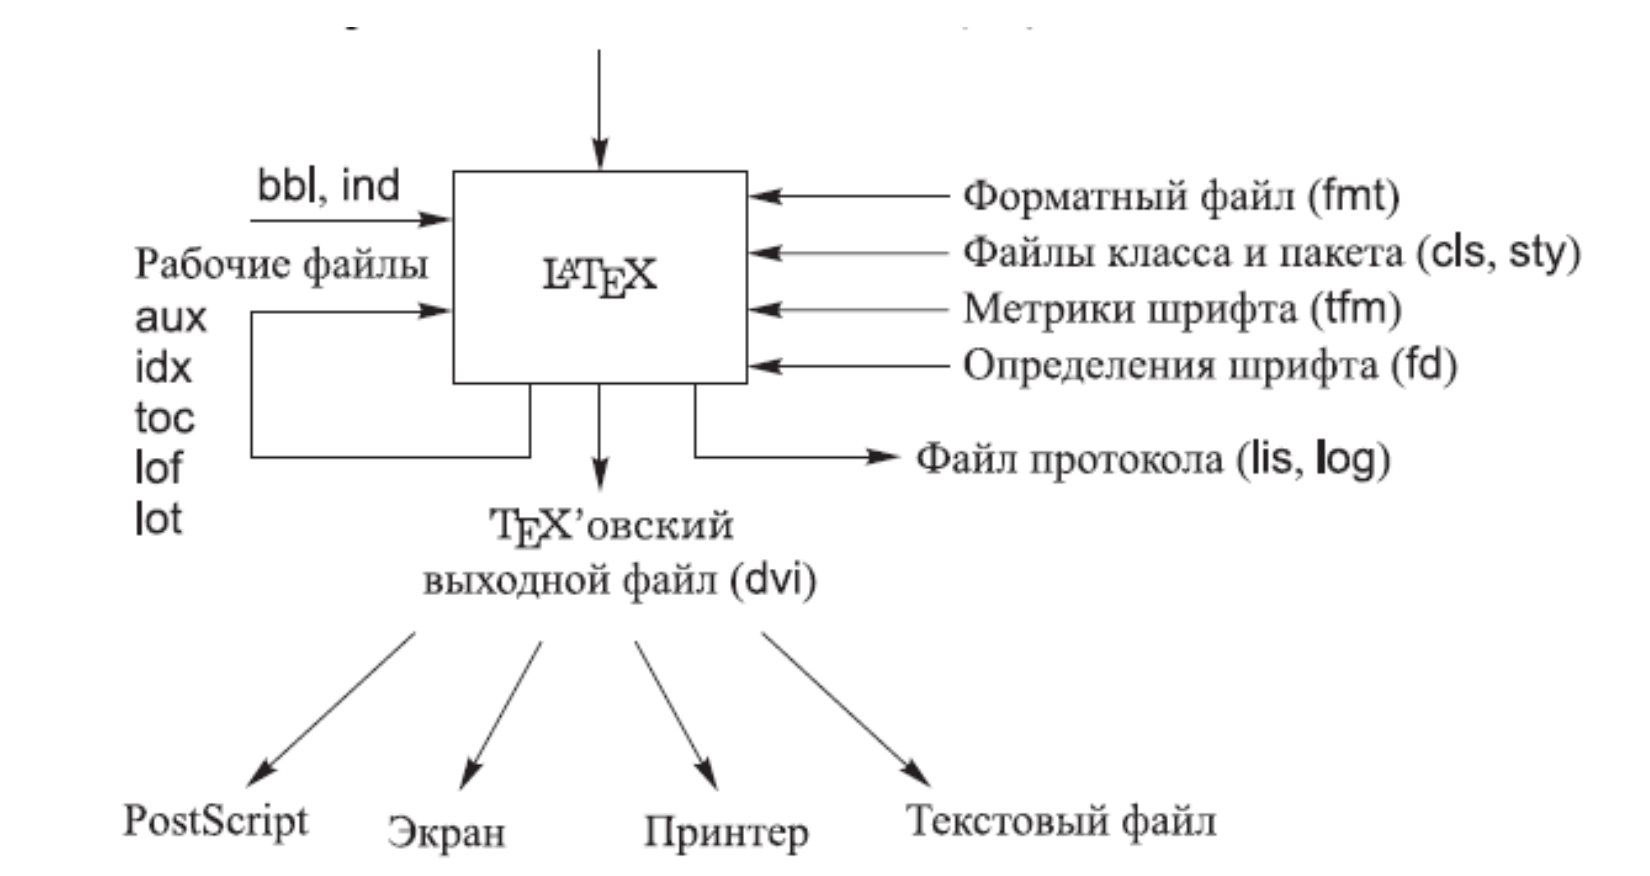
\includegraphics[width=0.5\linewidth]{img-1.png}}% файл с рисунком должен находиться в той же директории, что и tex-файл, при этом в случае использования команды latex должен быть файл ps или eps, при использовании команды pdflatex - png или jpg
    \caption{Рис. 1 — Схематическое описание процесса создания документа.} % подпись к рисунку
	\label {fig_1} % добавляем метку для дальнейшей ссылки на этот рисунок
\end{figure}


\section{Добавление таблиц и подписей к ним}

\begin{table}[!h] % выполните набор любой таблицы из лабораторной работы 3
	\centering % центрирование объекта
	\caption{Распространённость версий Windows по данным различных источников} \label{tab_1} % добавляем метку для дальнейшей ссылки на эту таблицу
    \begin{tabular}{ |*{4}c| } % укажите количество столбцов в вашей таблице и способ выравнивания текста в них
		 \hline
            & \textbf{«GoStats.ru», июнь 2011} & \textbf{«Net Market Share»,июнь 2011} & \textbf{«GoStats.ru»,август 2014} \\ 
		 \hline
         \textbf{Все версии} & 94,70 \% & 93,32 \% & 73,55\% \\
 		 \hline
         \textbf{Windows 10} & N/A & N/A & N/A \\ 
		 \hline
         \textbf{Windows 8} & N/A & N/A & 1,91\% \\ 
		 \hline
         \textbf{Windows 7} & 25,89\% & 28,68\% & 53,92\% \\
		 \hline
         \textbf{Windows XP} & 55,44\% & 54,04\% & 13,57\% \\
		 \hline

  

	\end{tabular}
\end{table}

\section{Добавление перекрестных ссылок на объекты и библиографические описания}

В научных статьях, книгах и различных отчетах принято ввылаться на источники, которые вы цитируете или в которых то, о чем вы пишете в своем тексте, раскрыто более подробно. Также принято ссылаться на статьи или другие источники, содержащие описание каких-либо исследований в литературных обзорах для подкрепления ваших слов. В сислеме \LaTeX{} есть набор средств, позволяющий выполнять цитирование, в первую очередь это команда \cite{Harrison_Cosmology}, \cite{Michie2009}, \cite{Barchi_2020}, \cite{Lee2016},\cite{tag_1}, \cite{tag_2} более подробно мы похзнакомимся с принципами работы с ней в следующей лабораторной работе.

Также принято ссылаться в тексте на рисунки, таблицы, формулы и листинги программ, для этого все объекты должны иметь метку с уникальным именем, при вызове команды для выполнения перекрестных ссылок, вы подставляете в аргумент команды уникальную метку и \LaTeX{} проставляет нужный номер автоматичски. Ссылки выполняются следующим образом:

\begin{itemize}
	\item Ссылка на рисунок \ref{fig_1}.
	\item Ссылка на таблицу \ref{tab_1}.
	\item ссылка на формулу \eqref{eq_1}.
\end{itemize}

\addcontentsline{toc}{section}{Литература} % эта команда добавляет строку, соответствующую списку литературы в содержание

\bibliographystyle{gost780s.bst}
\bibliography{name.bib}

\begin{thebibliography}{1} % окружение, формирующее список библиографических описаний источников

\bibitem{Harrison_Cosmology}
{Harrison,~E.} Cosmology: The Science of the Universe~/ E.~Harrison.
  "---
\newblock USA: Cambridge University Press, March 16, 2000.

\bibitem{Lee2016}
{Lee,~C.-Y.} Generalizing pooling functions in convolutional neural
 networks: Mixed, gated, and tree. "---
\newblock 2015.

\bibitem{Barchi_2020}
Machine and deep learning applied to galaxy morphology - a comparative study~/
  P.~Barchi, R.~de~Carvalho, R.~Rosa et~al.~// {Astronomy and
  Computing}. "---
\newblock 2020. "---
\newblock Vol.~30. "---
\newblock P.~100334.

\bibitem{Michie2009}
Machine Learning, Neural and Statistical Classification~/ Ed. by D.~Michie,
  D.~J.~Spiegelhalter, C.~C.~Taylor, J.~Campbell. "---
\newblock USA: Ellis Horwood, 1995.

\end{thebibliography}	


\end{document}

